\chapter{Financial Planning and Investment}\label{ch:financial-planning}

I remember sitting with a talented entrepreneur from Boston who had an innovative AgriTech solution.\ ``Dele,'' he said, pulling out an impressively detailed financial model, ``I've planned everything down to the last naira.'' Looking at his numbers, I couldn't help but smile—he's thinking \$60,000 for his initial entry when he could have started effectively with \$30,000.

``Let me share something I learned while building Firmbird,'' I told him.\ ``In Nigeria, it's not about how much money you start with --- it's about how smartly you deploy it.''

\begin{importantbox}
When I helped that entrepreneur revise his plan, he ended up entering the market with half his original budget and achieved profitability in 23 months.\ This chapter will show you how to plan your finances similarly—efficiently and realistically.
\end{importantbox}

%2

\section{The Real Cost Structure}\label{sec:real-cost-structure}

When a UAE-based client asked about setup costs, I drew what I now call the ``Cost Triangle'':

\begin{figure}[h]
    \centering
    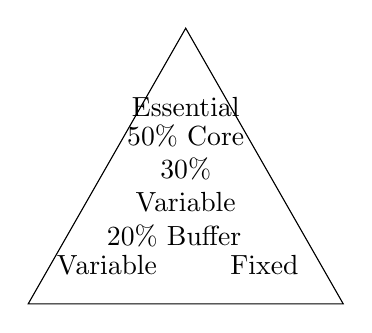
\begin{tikzpicture}
        % Cost Triangle visualization
        \draw (0,0) -- (4,0) -- (2,3.5) -- cycle;
        \node at (2,2.5) {Essential};
        \node at (1,0.5) {Variable};
        \node at (3,0.5) {Fixed};
        % Add percentages
        \node[text width=2cm] at (2,1.5) {\centering 50\% Core\\30\% Variable\\20\% Buffer};
    \end{tikzpicture}
    \caption{The Cost Triangle Framework}
    \label{fig:cost-triangle}
\end{figure}

Let's break this down into practical terms:

\subsection{Essential Setup Costs}\label{subsec:essential-setup-costs}
These are your non-negotiable startup expenses:

\begin{tcolorbox}[colback=white,colframe=primarydark,title=\textbf{Core Setup Components}]
\begin{itemize}
    \item \textbf{Legal \& Registration: \$2,000}
    \begin{itemize}
        \item Company registration
        \item Basic licenses
        \item Initial compliance
    \end{itemize}

    \item \textbf{Infrastructure: \$5,000-8,000}
    \begin{itemize}
        \item Office space (if needed)
        \item Basic equipment
        \item Utilities setup
    \end{itemize}

    \item \textbf{Technology: \$2,000-5,000}
    \begin{itemize}
        \item Core systems
        \item Essential software
        \item Basic security
    \end{itemize}

    \item \textbf{Initial Team: \$3,000-5,000}
    \begin{itemize}
        \item Essential personnel
        \item Basic training
        \item Initial payroll buffer
    \end{itemize}
\end{itemize}
\end{tcolorbox}

%3
\section{Monthly Operating Costs}\label{sec:monthly-operating-costs}

I always tell entrepreneurs, ``our first three months of operating costs aren't a cost --- they're part of your startup capital.'' Here's why:

\begin{center}
\begin{tabularx}{\textwidth}{>{\raggedright\arraybackslash}X >{\centering\arraybackslash}X >{\raggedright\arraybackslash}X}
    \toprule
    \textbf{Expense Category} & \textbf{Monthly Range} & \textbf{Notes} \\
    \midrule
    Staff & \$1,000-2,000 & Start lean, scale with revenue \\
    Infrastructure & \$500-1,000 & Location dependent \\
    Technology & \$200-500 & Based on business type \\
    Marketing & \$300-800 & Focus on targeted efforts \\
    Miscellaneous & \$200-500 & Always have a buffer \\
    \bottomrule
\end{tabularx}
\end{center}

\section{Revenue Projection Framework}\label{sec:revenue-projection}

A UK founder once asked me, ``Dele, how do I project revenues in a market I don't fully understand yet?'' I introduced her to what I call the ``Conservative Growth Ladder'':

\begin{tcolorbox}[colback=white,colframe=primarydark,title=\textbf{12-Month Revenue Framework}]
\begin{itemize}
    \item \textbf{Months 1--3: Establishment Phase}
    \begin{itemize}
        \item Focus on setup and initial clients
        \item Expect minimal revenue
        \item Target: Cover 20--30\% of operating costs
    \end{itemize}

    \item \textbf{Months 4--6: Growth Phase}
    \begin{itemize}
        \item Expand client base
        \item Optimize operations
        \item Target: Cover 50--60\% of operating costs
    \end{itemize}

    \item \textbf{Months 7--9: Stabilization Phase}
    \begin{itemize}
        \item Strengthen market position
        \item Increase efficiency
        \item Target: Cover 80--90\% of operating costs
    \end{itemize}

    \item \textbf{Months 10--12: Profitability Phase}
    \begin{itemize}
        \item Achieve stable operations
        \item Focus on profitability
        \item Target: Break-even or slight profit
    \end{itemize}
\end{itemize}
\end{tcolorbox}

\section{Leveraging Consumer Credit Reform Programs}\label{sec:consumer-credit}

One powerful tool that many entrepreneurs overlook is the new consumer credit reform programs.\ Let me tell you about two game-changing initiatives that can help extend your runway and speed up growth.

\subsection{The CALM Fund Opportunity}\label{subsec:calm-fund}

The Credit Access for Light and Mobility (CALM) Fund offers something particularly valuable for new market entrants.\ Here's how to leverage it effectively:

\begin{itemize}
    \item \textbf{Solar Energy Solutions}
    \begin{itemize}
        \item Finance your power infrastructure
        \item Reduce upfront costs by up to 60\%
        \item 24\% annual interest rate
        \item Up to 2-year repayment terms
    \end{itemize}

    \item \textbf{Transportation Solutions}
    \begin{itemize}
        \item CNG conversion financing
        \item Reduce operational costs
        \item Improve sustainability metrics
    \end{itemize}
\end{itemize}

\subsection{The SCALE Program Advantage}\label{subsec:scale-program}

The Securing Consumer Access to Local Enterprises (SCALE) Program can be a powerful ally in your growth strategy.\ Here's how to make it work for you:

\begin{itemize}
    \item \textbf{Digital Infrastructure}
    \begin{itemize}
        \item Access to digital devices
        \item Technology infrastructure support
        \item Reduced upfront costs
    \end{itemize}

    \item \textbf{Essential Equipment}
    \begin{itemize}
        \item Office setup financing
        \item Production equipment access
        \item Flexible payment terms
    \end{itemize}
\end{itemize}

%4
\section{Funding Sources and Strategies}\label{sec:funding-sources}

When it comes to funding your Nigerian market entry, I always share what I call the ``4S Framework'':

\begin{center}
\begin{tabularx}{\textwidth}{>{\raggedright\arraybackslash}X >{\centering\arraybackslash}X >{\raggedright\arraybackslash}X}
    \toprule
    \textbf{Source} & \textbf{Typical Range} & \textbf{Best For} \\
    \midrule
    Self-Funding & \$15,000-30,000 & Quick start, full control \\
    Silent Partners & \$25,000-50,000 & Expanded capacity \\
    Strategic Investors & \$30,000-75,000 & Market access \\
    Staged Investment & \$20,000-40,000 & Risk management \\
    \bottomrule
\end{tabularx}
\end{center}

\begin{warningbox}
I've seen too many entrepreneurs get caught in what I call the ``Big Money Trap'' --- raising more than they need and losing focus.\ Start with what you need, not what you can get.
\end{warningbox}

\section{Interactive Financial Planning Tools}\label{sec:financial-tools}

To help you plan your finances more effectively, we've created interactive financial planning calculators and templates.\ These tools will help you:

\begin{itemize}
    \item Model different scenarios
    \item Understand cost breakdowns
    \item Project cash flows
    \item Plan contingencies
\end{itemize}

You can download these resources at \href{https://viz.li/csl-book-ngbiz}{viz.li/csl-book-ngbiz}

\section{Workshop: Your Financial Plan}\label{sec:workshop}

\begin{workshopbox}
\textbf{Financial Planning Exercise}

1. Capital Requirements
\begin{itemize}
    \item Core setup costs: \_\_\_\_\_\_\_\_\_
    \item Operating buffer: \_\_\_\_\_\_\_\_\_
    \item Growth capital: \_\_\_\_\_\_\_\_\_
\end{itemize}

2. Monthly Budget
\begin{itemize}
    \item Fixed costs: \_\_\_\_\_\_\_\_\_
    \item Variable costs: \_\_\_\_\_\_\_\_\_
    \item Revenue targets: \_\_\_\_\_\_\_\_\_
\end{itemize}

3. Funding Strategy
\begin{itemize}
    \item Primary source: \_\_\_\_\_\_\_\_\_
    \item Backup options: \_\_\_\_\_\_\_\_\_
    \item Staged planning: \_\_\_\_\_\_\_\_\_
\end{itemize}
\end{workshopbox}

\begin{communitybox}
Connect with fellow entrepreneurs and access additional resources at \href{https://viz.li/csl-book-ngbiz}{viz.li/csl-book-ngbiz}:
\begin{itemize}
    \item Financial modeling templates
    \item Budgeting tools
    \item Funding source directory
    \item Expert advisory sessions
\end{itemize}
\end{communitybox}

\begin{importantbox}
Remember, successful market entry isn't about having the most money --- it's about having enough money and using it wisely.\ In the next chapter, we'll explore how to protect your investment through effective risk management and compliance.

With projected GDP growth of 4.12\% in 2025 and significant banking sector reforms underway, the timing for market entry has never been better.\ However, success depends not on timing alone, but on thorough preparation and strategic execution.\ In Chapter 6, we'll explore how to protect your investment through effective risk management.
\end{importantbox}